\documentclass[10pt]{article}
\usepackage{amsmath,amsthm}
\usepackage{amssymb}
\usepackage{anysize}
\usepackage{listings}
\usepackage{graphicx}

\usepackage[italian]{babel}

\usepackage{booktabs}
\usepackage[italian]{cleveref}

\usepackage{siunitx}

\usepackage{xcolor}

\definecolor{Blue}{rgb}{0.2,0.2,0.9}
\definecolor{Green}{rgb}{0,0.6,0}
\definecolor{Gray}{rgb}{0.5,0.5,0.5}
\definecolor{Purple}{rgb}{0.58,0,0.82}
\definecolor{background}{rgb}{0.98,0.98,0.95}

\lstdefinestyle{mystyle}{
    backgroundcolor=\color{background},   
    commentstyle=\color{Green},
    keywordstyle=\color{Blue},
    numberstyle=\tiny\color{Gray},
    stringstyle=\color{Purple},
    basicstyle=\ttfamily\footnotesize,
    breakatwhitespace=false,         
    breaklines=true,                 
    captionpos=b,                    
    keepspaces=true,                 
    numbers=left,                    
    numbersep=5pt,                  
    showspaces=false,                
    showstringspaces=false,
    showtabs=false,                  
    tabsize=2
}


\lstset{style=mystyle}


\renewcommand{\vec}[1]{\boldsymbol{#1}}
\newcommand{\tens}[1]{\mathsf{#1}}
\newcommand{\pd}[2]{\frac{\partial #1}{\partial #2} }
\newcommand{\HALF}{\frac{1}{2}}
\newcommand{\DS}{\displaystyle}

\newcommand{\im}[1]{\textsc{#1}}

\newcommand{\et}{\wedge}
\newcommand{\orr}{\vee}
\newcommand{\cond}{\middle|}
\newcommand{\lp}{\left}
\newcommand{\rp}{\right}
\newcommand{\pare}[1]{\left(#1\right)}

\theoremstyle{definition}
\newtheorem{example}{Esempio}[section]
\crefname{example}{Esempio}{Esempi}

\theoremstyle{definition}
\newtheorem{property}{Proprietà}[subsection]
\crefname{property}{Proprietà}{Proprietà}

\DeclareMathOperator{\pr}{Pr}


\begin{document}

\title{Note del corso\\\textsc{Machine Learning per la fisica applicata\\e fisica delle alte energie}}
\author{Raviola Alessio}
\date{\today}

\maketitle

%%%%%%%%%%%%%%%%%%%%%%%%%%%%%%%%%%%%%%%%%%%%%%%%%%%%%%%%%%%%%%%%%%%%%%%%
\section{Introduzione}
%
%
%%%%%%%%%%%%%%%%%%%%%%%%%%%%%%%%%%%%%%%%%%%%%%%%%%%%%%%%%%%%%%%%%%%%%%%%
\begin{quotation}
A computer program is said to learn from experience E with respecto to some class of tasks T and performance measure P, if its performance at tasks in T, as measured by P, improves with experience E.
\end{quotation}
L'impostazione del corso è di tipo \textit{probabilistico} (statistical learning). Le quantità non note sono trattate come \textbf{variabili aleatorie} (\im{random variables}) a cui viene associata una \textbf{distribuzione di probabilità} (\im{probability distribution}) che descrive il set (pesato) di valori che la variabile può assumere.

Abbiamo tre tipi di machine learning:
\begin{itemize}
\item \im{supervised learning};
\item \im{unsupervised learning};
\item \im{reinforcement learning};
\end{itemize}
il corso si focalizza sui primi due tipi.

\subsection{Supervised learning}
Il \textbf{compito} T consiste nell'imparare una mappa $f$ dagli input $x\in X$ agli output $y\in Y$. Gli \textbf{input} $x$ sono chiamati \im{features} (o \im{covariates} o \im{predictors}) e sono in genere costituiti da un vettore reale con dimensione fissata, ovvero abbiamo $X\equiv \mathbb{R}^D$. Gli \textbf{output} sono chiamati \im{label} (o \im{target} o \im{response}).

L'\textbf{esperienza} E consiste in un \im{training set} $\mathcal{D}$ di $N$ coppie input-output:
\begin{equation}
\mathcal{D} = \left\{ (x_n, y_n) \right\}_{n=1}^N,
\end{equation}
dove $N$ è detta \im{sample size}.

La \textbf{performance} dipenda dal compito T.

\subsubsection{Classificazione}
Problemi comuni in machine learning sono quelli di \textbf{classificazione}. In un problema di questo tipo lo spazio degli output C è un set \textit{non ordinato} di label $y = \{ 1, 2, \cdots, C \}$ dette \im{classes}. Quello che chiede il problema è di predire una classe dato un input, problemi di questo tipo sono detti di \im{pattern recognition}\footnote{Se abbiamo solo due classi, i.e. solo due output, allora il problema si dice di \im{classificazione binaria}}.

\begin{example}[Classificazione specie di iris]
In generale in \im{image classification} gli input $X$ sono immagini, quindi:
\begin{equation}
X = R^D,\quad D = C\times D_1\times D_2,
\end{equation}
ove $C = 3$ sono i canali RGB. E cerchiamo una mappa
\begin{equation}
f: X \longrightarrow Y
\end{equation}
che ci dica a quale delle classi appartenenti a $Y$ l'immagine appartiene. Per le specie di iris però i botanisti hanno individuato 4 caratteristiche numeriche: lunghezza e larghezza del sepalo e del petalo; dunque abbiamo $X = \mathbb{R}^4$. Supponiamo che il traning set sia una collezione di 150 esempi delle 3 specie, 50 per ognuna. I dati possono essere raccolti in una matrice detta \im{design matrix} come \im{tabular data} - come in \Cref{tab:iris}.

\begin{table}
\centering
\begin{tabular}{rrrrrl}
\toprule
Index & sl [cm] & sw [cm] & pl [cm] & pw [cm] & Label \\
\midrule
0 & 5.1 & 3.5 & 1.4 & 0.2 & Setosa \\
1 & 4.9 & 3.0 & 1.4 & 0.2 & Setosa \\
\vdots & \vdots & \vdots & \vdots & \vdots & \vdots \\
50 & 7.0 & 3.2 & 4.7 & 1.4 & Versicolor \\
\vdots & \vdots & \vdots & \vdots & \vdots & \vdots \\
150 & 5.9 & 3.0 & 5.1 & 1.8 & Virginica \\
\bottomrule
\end{tabular}
\caption{Design matrix del training set per classificazione specie di iris.}\label{tab:iris}
\end{table}

Se abbiamo $N$ elementi nel training set, ognuno con dimensione $D = \dim{X} + \dim{Y}$, allora abbiamo:
\begin{itemize}
\item \im{big data} se $N\gg D$, ovvero se il numero di elementi è molto superiore alla loro dimensione;
\item \im{wide data} se $D\gg N$, ovvero se la dimensione degli elementi è molto superiore al loro numero.
\end{itemize}

Una buona idea è fare una \textit{esplorazione dei dati} (\im{exploatory data analysis}) per vedere se ci sono dei pattern ovvi, ad esempio tramite grafici. Per grandi basi dati (big data) possiamo procedere mediante \im{dimensionality reduction}:
\begin{equation}
f(\vec{x}, \vec{\theta}) = \left.\begin{array}{l}
\left\{\begin{array}{ll}
p_l < \qty{2.45}{cm} & \text{Setosa} \\
\text{Altrimenti} & \left\{\begin{array}{ll}
p_w < \qty{1.75}{cm} & \text{Versicolor} \\
\text{Altrimenti} & \text{Virginica} \\
\end{array}\right.
\end{array}\right.
\end{array}\right\} \quad\text{\im{decision tree}},
\end{equation}
ove $\vec{\theta}$ è detto \im{threshold parameter}. Questo decision tree è visualizzato in \Cref{fig:iris-decision-tree}. La performance può essere quindi misurata con il \im{miscalssification rate}:
\begin{equation}
\mathcal{L}(\theta) \equiv \frac{1}{N}\sum_{n=1}^N \mathbb{I}\left( y_n \neq f(\vec{x_n}, \vec{\theta}) \right),
\end{equation}
dove $\mathbb{I}(e)$ è l'\textbf{indicatore binario}
\begin{equation}
\mathbb{I}(e) = \left\{\begin{array}{l@{\text{ se } e \text{ è }}l}
1 & \text{vero} \\
0 & \text{falso} \\
\end{array}\right..
\end{equation}
Nel caso in cui alcuni errori di classificazione siano più dannosi di altri posso definire una less function $l(y, \hat{y})$ e ridefinire il misclassification rate come l'\im{empirical risk}:
\begin{equation}
\mathcal{L}(\theta) \equiv \frac{1}{N}\sum_{n=1}^N l\left( y_n, f(\vec{x_n}, \vec{\theta}) \right).
\end{equation}
Un modo che abbiamo per definire il \im{training} (o \im{model fitting}) è modificare questo rischio empirico, ovvero trovare $\hat{\theta}$ tale che
\begin{equation}
\mathcal{L}(\hat{\theta}) = \min[\mathcal{L}(\theta)].
\end{equation}

\begin{figure}
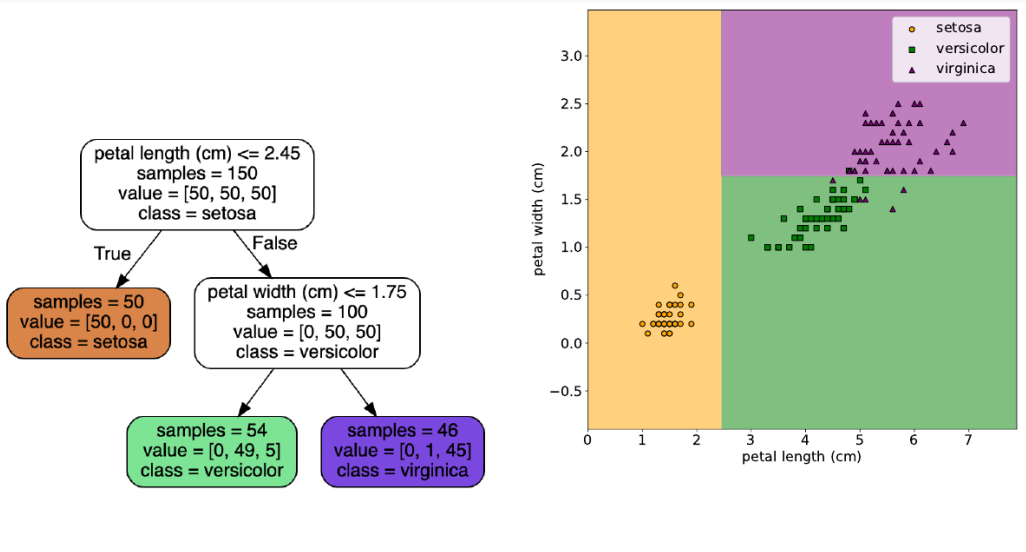
\includegraphics[width=0.98\textwidth]{Images/iris_decision_tree.PNG}
\caption{Decision tree per problema di classificazione specie di iris.}\label{fig:iris-decision-tree}
\end{figure}

\end{example}

\section{Richiami di probabilità}
Abbiamo diverse definizioni di probabilità.
\begin{description}
\item[Definizione Frequentistica] La probabilità di un evento è il rapporto tra il numero di casi favorevoli e il numero di casi possibili.
\item[Definizione Soggettiva] La probabilità di un evento è il prezzo che un individuo ritiene equo pagare per ricevere 1 se l'evento si verifica e 0 altrimenti.
\item[Definizione Bayesiana] La probabilità di un evento è l'\textit{incertezza} con cui l'evento si verifica.
\item[Definizione Assiomatica] Kolmogorov nel 1933 costruisce la teoria della probabilità a partire da degli assiomi.
\end{description}

L'incertezza può essere di due tipi:
\begin{description}
\item[aleatoria] ovvero è una \im{data uncertanty};
\item[epistemica] ovvero è una \im{model uncertanty};
\end{description}

\subsection{Proprietà della probabilità}
Chiamiamo $\pr(A)$ la probabilità dell'evento $A$, allora abbiamo le seguenti proprietà.

\begin{property}[Joint probability]
Se $A$ e $B$ sono due eventi indipendenti, allora:
\begin{equation}
\pr(A\et B) \equiv \pr(A, B) = \pr(A) \cdot \pr(B).
\end{equation}
\end{property}

\begin{property}[Union probability]
Anche detta regola di unione esclusione. Se $A$ e $B$ sono due eventi indipendenti, allora:
\begin{equation}
\pr(A\orr B) = \pr(A) + \pr(B) - \pr(A\et B).
\end{equation}
\end{property}

\begin{property}[Conditional probability]
\begin{equation}
\pr(A\mid B) = \frac{\pr(A, B)}{\pr(A)}.
\end{equation}
Se i due eventi sono indipendenti questa si riduce a $\pr(A\mid B) = \pr(A)$.
\end{property}

\begin{property}[Conditional independece]
\begin{equation}
\pr(A, B \mid C) = \pr(A\mid C) \cdot \pr(B\mid C)
\end{equation}
\end{property}

\subsection{Random variables}
Rappresentiamo con $X$ una variabile di cui non conosciamo il valore e la chiamiamo \textit{variabile casuale} (\im{random variable}). Il set dei valori che $X$ può assumere è detto \textit{spazio di sampling} (\im{sampling space}). Un evento è dunque un set di risultati dato un sampling space definito.

Se la variabile è \textbf{discreta} abbiamo un sampling space numerabile e la PMF (\im{probability mass function}):
\begin{equation}
p(x) \equiv \pr(X = x).
\end{equation}
Se invece la variabile è \textbf{continua} abbiamo un samplig space non numberabile e la CDF (\im{cumulative distribution function}):
\begin{equation}
P(x) \equiv \pr(X \leq x),
\end{equation}
da cui possiamo definire la PDF (\im{probability density function}):
\begin{equation}
p(x) \equiv \frac{d}{dx}P(x),
\end{equation}
da cui segue:
\begin{align}
&\pr(a \leq X \leq b) = \int_a^b p(x) = P(b) - P(a) \\
&\Longrightarrow \pr(x \leq X \leq x + dx) \approx p(x).
\end{align}
Se la CDF $P(x)$ è monotona crescente allora la sua inversa $P^{-1}(q)$ è detta \textit{quantile}. Il valore $x_q = P^{-1}(q)$ è il valore per cui $\pr(X\leq x_q) < q$, ovvero il quantile $q$ della distribuzione $P$.

Se abbiamo due variabili casuali $X$ e $Y$ allora possiamo definire la \im{joint distribution}:
\begin{equation}
p(x, y) = p(X = x, Y = y) \equiv p(X = x\et Y = y).
\end{equation}
Se le due variabili sono indipendenti e con cardinalità finita possiamo definire la \textit{distribuzione marginale} (\im{marginal distribution}) come:
\begin{equation}
p\pare{X = x} = \sum_y p\pare{X=x, Y=y},
\end{equation}
altrimenti se sono dipendenti la \textit{distribuzione condizionale} (\im{conditional distribution}) come:
\begin{equation}
\begin{split}
&p\pare{Y=y\cond X=x} = \frac{p\pare{X=x, Y=y}}{p\pare{X=x}} \\
&\Longrightarrow\quad p\pare{x, y} = p\pare{y\cond x}\cdot p\pare{x},
\end{split}
\end{equation}
da cui segue la \textbf{chain rule}:
\begin{equation}
p\pare{\vec{x}_1,D} = p\pare{x_1} p\pare{x_2\cond x_1} p\pare{x_3\cond x_1, x_2}\cdots p\pare{x_D\cond p_{1: D-1}}.
\end{equation}

Due variabili si dicono \im{marginalmente indipendenti} se
\begin{equation}
X\perp Y \quad\Longleftrightarrow\quad p\pare{X, Y} = p\pare{X} p\pare{Y},
\end{equation}
mentre si dicono \textbf{condizionalmente indipendenti} se
\begin{equation}
X\perp Y \quad\Longleftrightarrow\quad p\pare{X, Y\cond Z} = p\pare{X\cond Z} p\pare{Y\cond Z}. 
\end{equation}

\subsection{Momenti di una distribuzione}

\end{document}
